% Exercise ID: MAT_P4FUNCOE_4FIN_GRA_005
% Exercise ID: MAT_P4FUNCOE_4FIN_GRA_005
% Module: MÓDULO P4 - Funções | Concept: Função Inversa | Type: Determinação Gráfica
% Difficulty: 2/5 (Fácil) | Type: desenvolvimento
% Points: 10 | Time: 10 min
% Tags: inversa, grafico, simetria, funcao_quadratica
% Author: Professor | Date: 2025-11-18
% Status: active
% Description: Dado o gráfico de ramos de funções, desenhar o gráfico da inversa

\exercicio
Na figura está representado o gráfico de uma função $f$ definida em $[-2, 2]$. Represente, no referencial dado, o gráfico da função inversa $f^{-1}$.

\begin{figure}[ht]
\centering
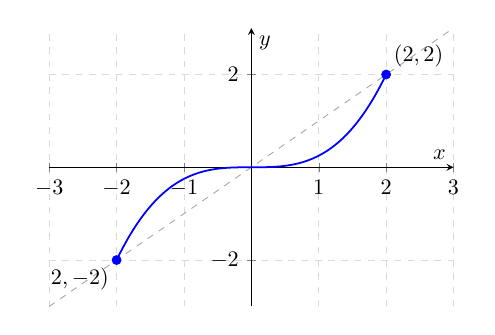
\begin{tikzpicture}[scale=0.8]
    \begin{axis}[
        axis lines = middle,
        xlabel = $x$,
        ylabel = $y$,
        xmin = -3, xmax = 3,
        ymin = -3, ymax = 3,
        grid = major,
        grid style = {dashed, gray!30},
        width = 8cm,
        height = 6cm,
    ]
    \addplot[domain=-3:3, dashed, gray!70, thin] {x};
    
    \addplot[domain=-2:2, samples=100, thick, blue] {x^3/4};
    \addplot[mark=*, mark size=2pt, blue] coordinates {(-2,-2)};
    \addplot[mark=*, mark size=2pt, blue] coordinates {(2,2)};
    \node[anchor=north east] at (axis cs:-2,-2) {$(-2,-2)$};
    \node[anchor=south west] at (axis cs:2,2) {$(2,2)$};
    \end{axis}
\end{tikzpicture}
\end{figure}

\bigskip

\exercicio
Na figura está representado o gráfico de uma função $g$ definida em $[0, 3]$. Represente, no referencial dado, o gráfico da função inversa $g^{-1}$.

\begin{figure}[H]
\centering
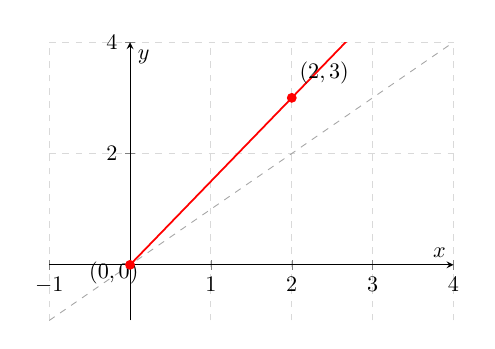
\begin{tikzpicture}[scale=0.8]
    \begin{axis}[
        axis lines = middle,
        xlabel = $x$,
        ylabel = $y$,
        xmin = -1, xmax = 4,
        ymin = -1, ymax = 4,
        grid = major,
        grid style = {dashed, gray!30},
        width = 8cm,
        height = 6cm,
    ]
    \addplot[domain=-1:4, dashed, gray!70, thin] {x};
    
    \addplot[domain=0:3, thick, red] {3*x/2};
    \addplot[mark=*, mark size=2pt, red] coordinates {(0,0)};
    \addplot[mark=*, mark size=2pt, red] coordinates {(2,3)};
    \node[anchor=south west] at (axis cs:2,3.1) {$(2,3)$};
    \node[anchor=north east] at (axis cs:0.2,0.2) {$(0,0)$};
    \end{axis}
\end{tikzpicture}
\end{figure}
\vspace{3cm}
}